% Here is a suggested template for PhD research proposal for the
% first annual report.
% Written originally 2010-06-22 by T. W. Yee.
% Last modified      2010-07-22 by T. W. Yee.

\documentclass[12pt,a4paper]{article}

\usepackage{natbib}    % For BibTeX
\usepackage{graphicx}  % To import .pdf files
\usepackage{caption}
\usepackage{subcaption}
\usepackage{booktabs}
\usepackage{comment}
% \usepackage{times}
\usepackage{setspace}
\onehalfspacing
% \doublespacing

\oddsidemargin  -10mm
\evensidemargin -10mm
\headheight 0mm
\headsep -3mm
\textheight 250mm
\textwidth 180mm
\topmargin -4mm
\topskip -10mm

%\textwidth=450pt
%\hoffset=-2cm


\usepackage{amsmath}
\usepackage{amsfonts}
\newcommand{\bu}{\boldsymbol{u}}
\newcommand{\bx}{\boldsymbol{x}}
\newcommand{\by}{\boldsymbol{y}}
\newcommand{\bz}{\boldsymbol{z}}
\newcommand{\bY}{\mathbf{Y}}
\newcommand{\bX}{\mathbf{X}}
\newcommand{\bZ}{\mathbf{Z}}
\newcommand{\btheta}{\boldsymbol{\theta}}
\newcommand{\mat}[1]{\mathbf{#1}}

\usepackage[acronym]{glossaries}
\newacronym[shortplural={ATIS}]{atis}{ATIS}{advanced traveller information system}
\newacronym{avl}{AVL}{automatic vehicle location}
\newacronym{apc}{APC}{automatic passenger counter}
\newacronym{rti}{RTI}{real-time information}
\newacronym{gps}{GPS}{Global Positioning System}
\newacronym{api}{API}{application programming interface}
\newacronym{gtfs}{GTFS}{general transit feed specification}
\newacronym{knn}{KNN}{$k$-nearest neighbour}
\newacronym{ann}{ANN}{artificial neural networks}
\newacronym{svm}{SVM}{support vector machines}
\newacronym{kf}{KF}{Kalman filter}
\newacronym{pf}{PF}{particle filter}
\newacronym{mcmc}{MCMC}{Markov chain Monte Carlo}
\newacronym[longplural={expected times of arrival}]{eta}{ETA}{expected time of arrival}
\newacronym{at}{AT}{Auckland Transport}
\newacronym{pt}{PT}{public transport}
\newacronym{ui}{UI}{user interface}
\newacronym{sir}{SIR}{sampling importance resampling}

\newcommand{\kf}{Kalman filter}
\newcommand{\pf}{particle filter}


\usepackage{tikz}

%\definecolor{mDarkBrown}{HTML}{604c38}
%\definecolor{mDarkTeal}{HTML}{23373b}
%\definecolor{mLightBrown}{HTML}{EB811B}
%\definecolor{mLightGreen}{HTML}{14B03D}
% \definecolor{mDarkBrown}{HTML}{8A7B71}
% \definecolor{mDarkTeal}{HTML}{EFECE1}
% \definecolor{mLightBrown}{HTML}{DCB190}
% \definecolor{mLightGreen}{HTML}{B8D38C}
\definecolor{mDarkBrown}{HTML}{FFFFFF}
\definecolor{mDarkTeal}{HTML}{FFFFFF}
\definecolor{mLightBrown}{HTML}{FFFFFF}
\definecolor{mLightGreen}{HTML}{FFFFFF}

\usetikzlibrary{shapes.geometric, arrows}
\tikzset{font=\scriptsize}
\tikzstyle{startstop} = [rectangle, rounded corners, minimum width=2.7cm,%
minimum height=0.6cm, text centered, draw=black, fill=mLightBrown!50]
\tikzstyle{compute} = [rectangle, minimum width = 2.7cm, minimum height = 0.7cm,%
text centered, draw=black, fill=mLightGreen!40]
\tikzstyle{logic} = [diamond, minimum width = 1.2cm,%
text centered, draw=black, fill=mDarkTeal]
\tikzstyle{data} = [circle, minimum width=0.5cm,text centered,%
draw=black,fill=white]
\tikzstyle{arrow} = [thick,->,>=stealth]
\tikzstyle{line} = [thick]




\usepackage{varioref}
\usepackage[hidelinks]{hyperref}
\usepackage[noabbrev]{cleveref}



\begin{document}

\begin{Large}
\begin{center}
\textbf{Real-time prediction of bus arrival} \\
\textbf{by Tom Elliott} \\
\textbf{for a PhD in Statistics}
\end{center}
\end{Large}


\hfill{Student ID: 1596870}

\hfill{Email: tom.elliott@auckland.ac.nz}

Supervisor: Professor~T.~Lumley

% Co-supervisor: Dr~B.~Brewer

% Advisory Committee: Drs~B.~Efron, D.~R.~Cox, K.~Pearson.\footnote{
% Specify the affiliation if outside the UoA Statistics
% Department.}


\begin{center}
\today
\end{center}


This document represents the student's research proposal after
one year of provisional PhD registration.
Confirmed PhD registration is now sought.


\vspace{2em}
\noindent
The primary goal of our work is to develop a more robust modelling
and prediction framework to make improved predictions of bus arrival time.
The key components of this will be a particle filter for the state estimation,
and a real-time traffic state ``map'' based on the combined states of all buses in Auckland
to improve prediction accuracy.
We will also investigate the use of prediction intervals and journey planning applications
to make our predictions accessible to commuters.
%We will then investigate methods of making our predictions available to commuters,
%primarily through prediction intervals and journey planning applications.



% ----------------------------------------------------------------------
\section{Introduction}
\label{sec:intro}




In order to attract greater ridership, many public transport agencies have deployed \glspl{atis}
to make public transport a more appealing option for commutes.
One major component of \gls{atis} is provision of \gls{rti},
in particular arrival time,
which usually comes in the form of a countdown display at stops
\citep{tcrp:2003}.
Several studies have shown that in the presence of real-time arrival information,
passengers perceive shorter waiting times (time passes more quickly),
and are generally more accepting of having to wait at the bus stop
\citep{tcrp:2003b}.


While countdowns are perhaps the most obvious form of \gls{rti},
it can also be very useful for passengers planning their journey.
For example, they can find out before heading to the bus stop what time it is expected to arrive,
enabling them to time their arrival to reduce waiting time.
Additionally, they may need to arrive at their destination before (or after) a specific time,
so consulting \gls{rti} can help them in deciding which bus to catch.
This all becomes especially useful when there are significant delays in the system.


Of course, in order to provide \gls{rti},
transit companies first need to deploy certain technologies to make it possible.
The main technology responsible for \gls{rti} is \gls{avl},
which allows tracking of transit vehicles in real-time.
This location information can then be used to determine the state of a vehicle,
for example speed and position along a route,
which is in turn used to predict arrival times at stops further along the route.


Another use for \gls{avl} information is for developers of public transport apps,
such as the \emph{Track My Bus} app \citep{trackmybus},
which is yet another form of \gls{atis}.
One common way of making public data accessible to developers is through an \gls{api}.
Many transit \glspl{api} use \gls{gtfs}, 
which is a globally used format for providing transit data---%
including real-time vehicle locations---to developers,
and is used by Auckland Transport.


Over the years, many statistical models have been implemented using a variety of \gls{avl} technologies
targeting a range of different applications.
Early works, such as those of \cite{wall-dailey:1999} and \cite{dailey:2001},
used the \kf{}, which is ideal for real-time tracking and navigation applications,
due to its speed and low computational requirements.
Other research has focused on data-driven and machine-learning models,
most notably \gls{ann} and \gls{svm},
which were found to provide more accurate predictions for stops further ahead
than the \kf{}, which was only able to accurately predict a few stops ahead
\citep{chang-etal:2010}.


Recently, the \pf{} has been used in several transit operations research applications
\citep{chen-rakha:2014,hans-etal:2015}.
The key benefits of the \pf{} are that it allows a more explicit specification of the model
that requires far fewer assumptions than the \kf{},
allowing it to sample a more complete range of plausible states and
overcome many of the problems affecting other transit models,
at the cost of heavier computational demands.


Within the Auckland Transport system, there are several key issues we hope to overcome.
The first of these is prediction inaccuracy,
which typically presents as sudden changes in \glspl{eta}.
The underlying model estimating the actual position of transit vehicles needs improvement,
particularly in how it handles loops, in which, given a coordinate,
a bus could be either heading into or out of the loop,
as shown in \vref{fig:colwill-loop}.
In this case, the first instance (left) is the result of a poorly modeled vehicle position,
leading the passenger to believe that they have missed their bus.
Another problem is driver error, 
for example when entering the wrong route number or forgetting altogether,
which has obvious implications to models that rely on this information---%
while we cannot fix this, we need to be aware of it so we can make
allowances in our models.


\begin{figure}[bt]
  \centering
  \begin{subfigure}{0.35\textwidth}
    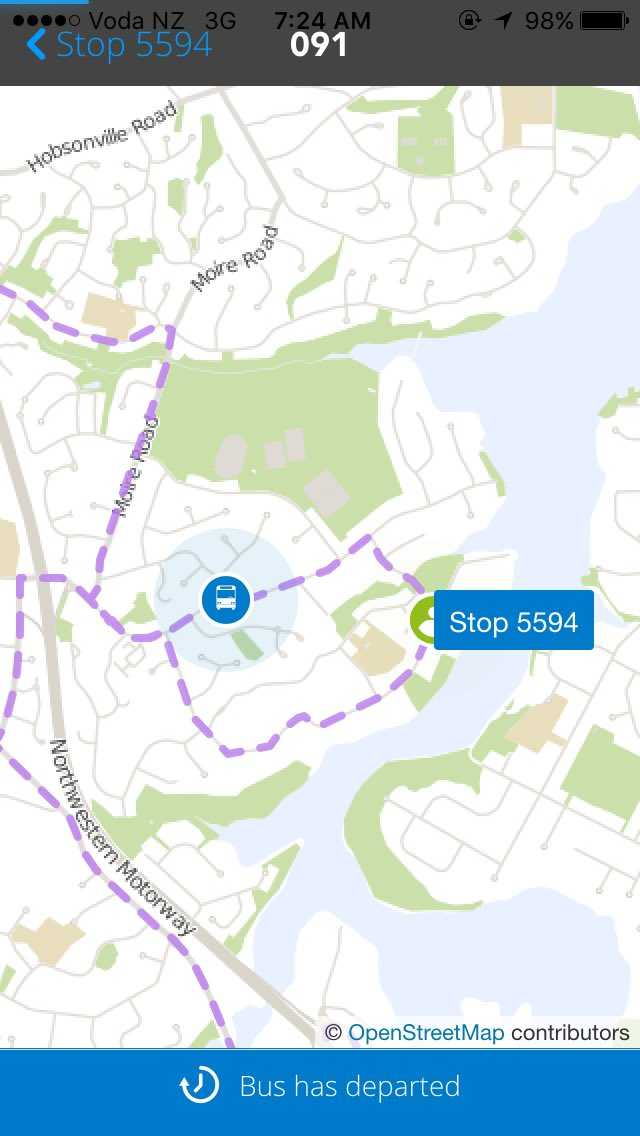
\includegraphics[width=\textwidth,trim={0 0 0 15cm},clip]{bus-loop-durp1.jpg}
    \caption{7:24~am}
    \label{fig:colwill-loop-1}
  \end{subfigure}
  ~
  \begin{subfigure}{0.35\textwidth}
    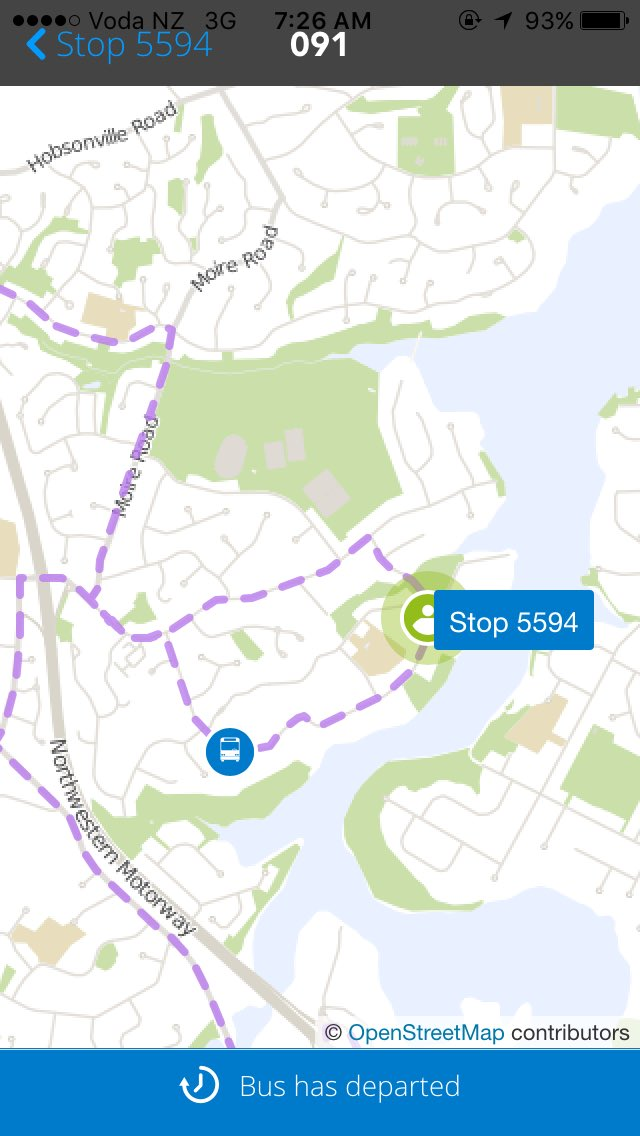
\includegraphics[width=\textwidth,trim={0 0 0 15cm},clip]{bus-loop-durp2.jpg}
    \caption{7:26~am}
    \label{fig:colwill-loop-2}
  \end{subfigure}
  \caption{%
    The scheduled arrival time at stop~5594 is 7:24~am,
    and the loop runs anti-clockwise.
    The bus position was wrongly estimated in (a),
    implying to the passenger that they had missed their bus.
    Note that in (b), even when the bus is later positioned correctly on the route,
    the status is still \emph{departed},
    which implies that the underlying model is unable to correct itself in this situation.\newline
    \footnotesize{[Screenshot taken from \emph{Track My Bus} \citep{trackmybus}].}}
  \label{fig:colwill-loop}
\end{figure}


Our primary goal is to implement a \pf{} to the \gls{avl} data provided by Auckland Transport
that can accurately model buses in Auckland,
while overcoming the issues mentioned above.
We will next explore ways of combining the real-time state of other buses in Auckland
to provide ``real-time'' traffic congestion information 
and increase the accuracy and precision of predictions.
Lastly, we will investigate several applications of our prediction model:
to provide useful prediction intervals to passengers
(who we assume to have no statistical knowledge),
and a journey planning application allowing passengers to enter their destination
and be informed as to the ``best'' route(s) to take.

% ====================================================================================================== % INFO

% This document is a template that can be edited by the student.
% Fill in the details as you go along and delete these instructions.
% Do have your research proposal scrutinized by your supervisor before
% submitting it to the department.



% Give a few paragraphs here on the general background
% to your research proposal; put the full details in
% Section~\ref{sec:background}. You might want to cite a few
% previous important results/papers. Describe any theory briefly
% here but put most of the details in Section~\ref{sec:background}.
% Describe any data in general with a few lines here but put the
% full details in Section~\ref{sec:data}.


% Motivate this section well \ldots why is the topic important?
% What use will the thesis have?
% What is unknown that will be known upon completion?


% This section should be understandable by an intelligent person
% who is not familiar with the technical details involved.
% The reader should be convinced that your work
% is worthwhile.





% Some of our PhD students have published in the primary literature
% directly using material from their thesis,
% e.g.,
% \cite{wors:1979},
% \cite{yee:wild:1996},
% \cite{wild:yee:1996},
% \cite{murr:1999},
% \cite{jian:scot:wild:2006},
% \cite{roev:meye:etal:2007},
% \cite{mill:stew:2007},
% or submitted such as
% \cite{lee:hiro:2008}.
% Ideally you should aim at least one of your publications towards
% a mainstream statistics journal, preferably your first one.
% All publications should be in a peer-reviewed international journal.
% It should be in the primary literature.
% Statistical theory and methodology is to be regarded as the highest
% form of quality output.
% Accompanying high quality software that can easily be used
% by others (such as a R package) is also good.
% It is best to submit to journals before the completion of a thesis
% because an acceptance validates the quality of that research.



% A word about writing up your thesis.
% In general, the Department of Statistics recommends \LaTeX{} rather than
% Microsoft Word.
% \LaTeX{} is easily run on the Department's Linux machines.
% A website that converts pdf into Word is \textsf{www.pdftoword.com}.
% The University of Auckland offers a half-day workshop
% on \LaTeX{} to postgraduate students.
% There is Sweave \citep{lmucs-papers:Leisch:2003b} which allows R
% \citep{R:Ihaka+Gentleman:1996} to be embedded into a \LaTeX{}
% document, and so the output does not have to be manually
% cut-and-pasted in. Sweave is useful for presentations too,
% in conjunction with Beamer.


% There is an editor called Emacs which is useful for all types of
% editing, including \LaTeX{}, C, and R.
% In Windows there is Tinn-R for R files and MiKTeX for \LaTeX{}.


% Note that {BibTeX} items are available from MathSciNet
% which is part of the ``Library Databases'' in the UoA electronic library
% system.
% There is a close relationship between EndNote and {BibTeX}.

% ----------------------------------------------------------------------

\section{Background}
\label{sec:background}

Ever since the first use of an \gls{avl} technology in 1964, in Hamburg, Germany,
it has become an integral part of most transit systems around the world
\citep{tcrp:1997,tcrp:2003}.
The first \gls{avl} systems used \emph{signpost} technology,
in which buses are fitted with a transponder that communicates with
sensors positioned along the route.
Other technologies include \emph{odometers},
which provide measurements of the distance traveled by a vehicle,
and more commonly in recent years the \gls{gps}.


In order to convert \gls{gps} coordinates into arrival time predictions,
several steps need to be taken.
The first of these is to estimate the \emph{actual state} of the bus,
for example its speed and how far into the route it has traveled---%
referred to as \emph{distance into trip}---%
which is often estimated directly from the \gls{gps} coordinates
(see \cref{sec:kalman-filter}),
and needs to account for \gls{gps} error.
The second step uses the estimated state
to predict how long the bus will take to travel from its current position
to a position farther along the route, usually a bus stop,
referred to as \emph{travel time};
given travel time and the current time, 
we can compute \emph{arrival time} at a stop.


In this section, we give an overview of some of the models that have been used
to generate real-time arrival time predictions,
with particular focus on Kalman and particle filtering.
We will briefly discuss some computer learning models which---%
although we will not be using them---%
cover important ground with respect to the important features of bus models.
Following this, we will describe in detail some of the
behaviours mentioned in the literature,
and finally discuss the difficulties associated with deploying many of these methods,
with particular mention of the type of data available.


\subsection{Real-time Bus Prediction}
\label{sec:history}

Over the last two decades,
there has been an enormous advance in both the technologies available and the models used
to track buses in real-time and simultaneously make arrival-time predictions for the upcoming stops.
Of particular interest are the recursive Bayesian filters,
namely the Kalman Filter, which has been used in transit models since the late 1990's,
and the particle filter, which has only recently shown up in the transit literature,
but has several unique characteristics we wish to exploit in our work.
In addition to these models,
there has also been a lot of progress in the field using data-oriented and machine learning models
such as \gls{knn}, \gls{ann}, and \gls{svm}.
We will briefly describe these,
focusing on the transit-specific features that were incorporated into them.



\subsubsection{Kalman Filter}
\label{sec:kalman-filter}

Given the real-time nature of the data, and the necessity for computations to be efficient,
recursive Bayesian filters are an obvious choice of model.
One popular filter that has been used in tracking and navigation,
as well as several bus-prediction applications,
is the \kf{} \citep{wall-dailey:1999,dailey:2001,shalaby-farhan:2004}.
As in all Bayesian recursive filters,
it assumes that there is an underlying, unmeasurable \emph{Markov process}
which has a state at time $k$ denoted $\bX_k$,
and an observable, dependent state for which we can obtain measurements $\bY_k$
\citep{jazwinski:1970}.
A \emph{measurement matrix}, $\mat{H}$,
or more generally a measurement function $h$,
describes the relationship between $\bX$ and $\bY$.


Modeling real-time data with any recursive Bayesian filter involves two steps:
\emph{predict} and \emph{update}.
In the predict step of the \kf{},
the Markov process is modeled using a \emph{transition matrix} $\mat{A}$
and Gaussian \emph{process noise} $\mat{w}_k \sim \mathcal{N}(0, \mat{G})$,
where $\mat{G}$ is a covariance matrix describing system noise.
The state is predicted using the model
\begin{equation}
  \label{eq:brf-predict}
  \hat\bX_k = \mat{A}_k \bX_{k-1} + \mat{w}_k.
\end{equation}
Next, in the update step, the state estimate is modeled using the equation
\begin{equation}
  \label{eq:brf-update}
  \bY_k = h(\bX_k) + \mat{e}_k,
\end{equation}
where $\mat{e}_k \sim \mathcal{N}(0, \mat{R})$,
and $\mat{R}$ is the covariance matrix describing measurement error.
The \kf{} algorithm generates a state estimate and associated covariance matrix
that is a trade-off between system noise and measurement error.
Since it uses only matrix operations,
it is a computationally efficient algorithm,
and is therefore suited to modeling data in real-time.


\cite{dailey:2001} formulated a \kf{} model using \gls{avl} data obtained by signposts and odometers,
which provided observations of \emph{distance traveled}, $\bar d_k$, and time.
To avoid confusion, we use $\mat{Z}$ for observations of \emph{distance},
that is $\mat{Z}_k = \left[ \bar d_k\ t_k \right]^T$;
$\bY$ will represent measurements from a \gls{gps} that we encounter later.
The true state was composed of distance into trip, speed, and the travel time
remaining to reach a given stop,
$\bX_k = \left[ d_k\ v_k\ \bar t_k \right]^T$.
Thus, assuming the odometer is reset at the beginning of each trip,
they used the measurement matrix $\mat{H} = \left[ 1\ 0\ 0 \right]$.
They used historical data to construct the
transition matrix at each step, and thus obtained a posterior
estimate of the new state which included time until arrival.


Unfortunately, the model implemented by \cite{dailey:2001} was not directly applicable
when the observations come from a \gls{gps}.
To overcome this, \cite{cathey-dailey:2003} proposed a general prescription
for making arrival time predictions from \gls{gps} data.
The main difference is in their first step, referred to as the tracker,
which involves estimation of the distance into trip from the reported \gls{gps} location;
that is, $\mat{Z}_k \approx g(\bY_k)$,
where $g$ is a map-matching algorithm.
Next, they assumed an unknown state consisting of distance into trip,
speed, and acceleration, $\bX_k = \left[ d_k\ v_k\ a_k \right]^T$,
and differential equations were used to generate the transition and covariance matrices.
The posterior state estimate, along with historical data,
was then used as an input to functions which made arrival time predictions,
rather than be estimated directly by the \kf{},
and the full prescription was demonstrated in Seattle and Orlando.


The model used by \cite{cathey-dailey:2003} first required the
estimation of $\mat{Z}_k$ from the observations,
which introduces an additional source of error.
We saw in \cref{fig:colwill-loop} what can happen when this is not done correctly.
Another related issue is that the \kf{} assumes multivariate normality
in all states, so in the situation displayed in \cref{fig:colwill-loop},
there is no way of temporarily allowing \emph{both} situations to be plausible,
which can lead to carry-on errors as in the figure (right)---%
the bus is still considered to have departed,
even after the position was corrected.



\subsubsection{Data-based models}
\label{sec:data-models}

Over the following decade, a range of modeling approaches were implemented, demonstrated,
and deployed in transit systems around the world.
These included \gls{knn}, in which real-time trips are matched to similar historical trips,
and computer learning models, most notably \gls{ann} and \gls{svm},
which use historical data sets to learn relationships between variables
which can then be used with real-time data to make predictions
\citep{park-rilett:1999,jeong-rilett:2005,yu-etal:2006,yu-etal:2010,yu-etal:2011}.
These, particularly \gls{svm}, usually gave more accurate arrival time
predictions than the \kf{}, and were not limited to only a few stops ahead.
More importantly, they allowed researchers to include more complex features
unique to transit vehicles.


Perhaps the most important feature recognised in transit models is \emph{dwell time}.
This is defined here as the \emph{time lost due to stopping at a bus stop},
which includes the deceleration and acceleration period of the bus.
The technical details are given later in \cref{sec:bus-behaviour}.
\cite{shalaby-farhan:2004} included dwell times in a \kf{} model,
although not explicitly,
and relied on the availability of \glspl{apc},
which provide estimates of the number of passengers boarding at each stop.
\cite{jeong-rilett:2005}
incorporated dwell times into an \gls{ann} model based on detailed \gls{avl} data
that also provided arrival and dwell times for visited stops.


Another feature of bus models is that, in many situations,
there are multiple trips along the same route every day,
and \cite{yu-etal:2006} developed an \gls{svm} model which used the travel time
of the preceding bus as one of the variables used to predict arrival time.
In many situations, such as in urban areas,
several routes may converge and use the same set of bus stops,
in which case it would be useful to use the most recent bus from \emph{any} route.
\cite{yu-etal:2011} implemented \kf{}, \gls{knn}, \gls{ann}, and \gls{svm} models that did just that,
of which the latter was found to provide the best results.
However, their data was based on automatic toll readers on the highway,
rather than \gls{avl},
so their model was limited in its scalability.



\subsubsection{Particle Filter}
\label{sec:particle-filter}

Recently, there has been some use of a \pf{} in transit applications,
which is another Bayesian recursive filter similar to the \kf{},
but with fewer assumptions and more flexibility.
Instead of modeling the entire state,
the \pf{}, originally named the ``bootstrap filter'' by  \cite{gordon-etal:1993},
uses a \emph{sample of particles} from the distribution,
each with its own state $\bX_k^{(i)}$.


In the predict step,
each particle is fed independently into a \emph{transition function}, $f$,
which can be as simple or detailed as necessary,
allowing the inclusion of process noise, $\sigma_v^2$,
as well as any other parameters for the necessary features 
(this is demonstrated in \cref{fig:pf_logic}):
\begin{equation}
  \label{eq:particle_transition}
  \bX_k^{(i)} = f(\bX_{k-1}^{(i)}, \sigma_v^2, \cdots).
\end{equation}
Since each particle is modeled independently,
there are no assumptions about the shape of the state distribution.


In the update step, each particle is assigned a weight, $w_i$, according to its likelihood
(which depends only on the observations and measurement error, $\sigma_y^2$):
\begin{equation}
  \label{eq:particle_weights}
  w_i = \frac{p(\bX_k^{(i)} | \bY_k, \sigma_y^2)}{\sum_{j=1}^M p(\bX_k^{(j)} | \bY_k, \sigma_y^2)}.
\end{equation}
The particles are then resampled with replacement according to their weights,
as in \gls{sir},
to obtain a sample from the posterior distribution \citep{gordon-etal:1993}.
Variations of (\ref{eq:particle_weights}) exist to increase the efficiency of the \pf{},
which we will likely need to consider when we begin
large-scale implementations of our model.


The likelihood for each particle is based on the distance between the particle
and the bus' reported \gls{gps} position.
Since each particle has its own value for the state parameters,
the distance into trip, $d_k^{(i)}$, can be transformed onto a geographic coordinate system
using the measurement function, $h$.
This is possible using the route shape information provided by \gls{gtfs} (\cref{sec:data}),
and is demonstrated in \cref{fig:gpsdist}.
The intermediate estimation of $\mat{Z}$ is no longer required,
which can help in overcoming situations where there are multiple plausible states:
in the loop example from earlier, some of the particles can be in one state
(heading into the loop, travelling slower), 
while the rest are in the other (heading out of the loop, travelling faster);
the posterior sample will be multimodal until a new observation is obtained to 
determine which state was true.

\begin{figure}[!b]
  \centering
  \begin{subfigure}{0.4\textwidth}
    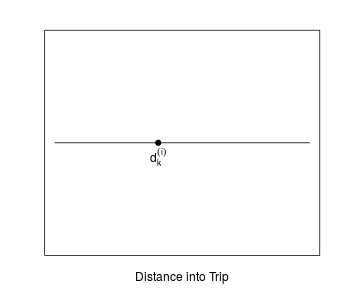
\includegraphics[width=\textwidth]{gps-dist2.png}
    %\caption{}
    \label{fig:gpsdist-1}
  \end{subfigure}
  ~
  \begin{subfigure}{0.4\textwidth}
    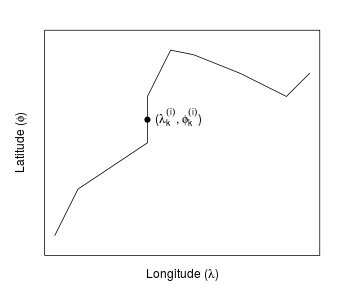
\includegraphics[width=\textwidth]{gps-dist1.png}
    %\caption{}
    \label{fig:gpsdist-2}
  \end{subfigure}
  \caption{%
  Each particle has a value for distance into trip, $d_k^{(i)}$ (left) which can be transformed
  into a geographic coordinate (right) using the shape information associated with
  the given route provided by \gls{gtfs}.}
  \label{fig:gpsdist}
\end{figure}

Being able to avoid unnecessary assumptions or estimations makes the
\pf{} a very attractive candidate for modeling real-time \gls{gps}-based data.
\cite{chen-rakha:2014} used a \pf{} to model travel time in real-time,
using historical data sets to propose new trajectories for particles.
\cite{hans-etal:2015} implemented one to model a transit system
in order to devise strategies
to reduce the bunching behavior of buses along the same route.
Their model included those features discussed in \cref{sec:data-models},
namely dwell times and travel times of previous trips.
Despite these few examples,
we have not seen evidence of \pf{} models deployed
to predict arrival times in real-time based solely on \gls{gps} locations provided
by \gls{gtfs}.



\subsection{Particulars of Bus Behaviour}
\label{sec:bus-behaviour}

Many of the models used in transit research were originally developed for 
more generic tracking applications or traffic state models;
however, there are several features that are unique to transit vehicles,
such as bus lanes and bus stops \citep{yu-etal:2011},
so models have needed adjusting accordingly.
The two which are of particular importance are dwell time and headway,
which have become a requirement in modern bus prediction methods
\citep{jeong-rilett:2005,hans-etal:2014,hans-etal:2015,cats-loutos:2016}.


Dwell time is defined as \emph{the total time lost due to stopping at a bus stop}.
This is shown visually in \cref{fig:dwell-time},
which shows the hypothetical paths of two vehicles, 
one of which stops while the other does not.
Therefore, there are two components to consider:
whether the bus stops, and if so, for how long.
The former can be expressed as a Bernoulli random variable, $p_j \sim \mathcal{B}(\pi_j)$,
where $\pi_j$, the average proportion of buses that stop,
is modeled according to the data available and the framework being used.


If a bus does stop, it must first decelerate,
and after servicing the bus stop it will take some time to accelerate back up to speed.
Additionally, there is time taken to open and close the doors.
These delays are usually combined into a common affect, $\gamma$,
as they apply to every bus and stop.
Once a bus has stopped, it will remain there while passengers board and disembark.
This can be modeled with an exponential distribution,
$\tau'_j \sim \mathcal{E}(\mu_\tau)$,
or else more complex queuing models can be constructed if the data allows
\citep{hans-etal:2015}.
The total dwell time experienced by the vehicle is $\tau_j = p_j(\gamma + \tau_j')$,
as shown in \cref{fig:dwell-time}.

\begin{figure}[bt]
  \centering
  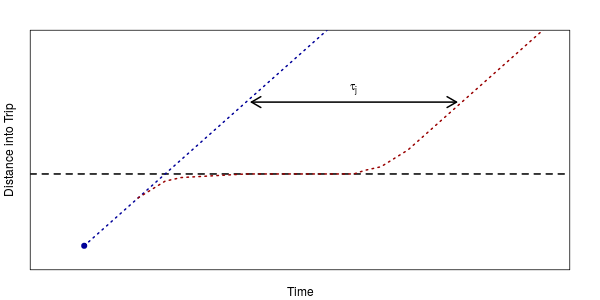
\includegraphics[width=0.8\textwidth]{dwell_time.png}
  \caption{Dwell time, $\tau_j$, is the total time lost due to stopping at a bus stop (indicated by the dashed black line).}
  \label{fig:dwell-time}
\end{figure}

The other important feature is headway,
which is the \emph{time delay between consecutive buses},
and can affect both travel times and dwell times.
If two consecutive routes are close together,
then the travel times are expected to be similar;
however, since they are both servicing the same route,
we expect the number of passengers waiting at a stop---and therefore
the dwell time---to be inversely proportional to the headway
\citep{hans-etal:2014,hans-etal:2015}.





\subsection{Availability of AVL Data}
\label{sec:data-types}

While there has been a lot of research in transit applications,
many of them have been concerned with operations control,
for example reducing bus bunching behaviour \citep{hans-etal:2015},
or else they require more informative data than is available in most systems,
such as \glspl{apc} and actual arrival times.
For the latter, it is usually because the \gls{avl} recording is triggered by stops
\citep{hans-etal:2015},
is high frequency \citep{chang-etal:2010},
or in some cases the test data was collected manually
\citep{yu-etal:2010}.


In Auckland's transport system, the only publicly available data is provided
by \gls{gps}, which is updated approximately every 30~seconds,
so arrival times must be estimated as latency variables and,
in a real-time deployment, will remain unknown.
Another issue specifically with Auckland Transport is that,
over the next few years,
the route structure is being completely redesigned
and rolled out slowly across the city.
Therefore, focus will be on using real-time and recent data (same day, week) to predict arrival times,
rather than relying on historical data collected over months or years.




% ====================================================================================================== % INFO

% Background knowledge is crucial, therefore describe it fully here.
% Specify the background to the problems you are trying to solve.
% Define anything technical that most statisticians will not be
% familiar with.

% What previous work has been done in the area?
% Cite references relating to such work, e.g.,
% in the form of \cite{reid:2003} and \cite{efro:tibs:1993}.
% Has anybody described any open problems in the literature?

% Make sure that problems arising from the background knowledge
% are clearly described. There should be a logical flow of thought
% in this section starting from the background and leading to the
% problem on hand.

% Don't put anything new in this section.

% ----------------------------------------------------------------------
\section{So What's New?}
\label{sec:whatsnew}

The primary goal of our work will be to develop a more robust modelling
and prediction framework to make improved predictions of bus arrival time.
The key components of this will be a particle filter for the state estimation,
and a real-time traffic state ``map'' based on states of all buses in Auckland
to improve prediction accuracy.
We will then investigate methods of making our predictions available to commuters,
primarily through the use of prediction intervals and journey planning applications.


\subsubsection*{Particle Filter State Model}

Our initial focus will be on formulating a particle filter to model the real-time state
of buses in Auckland,
with the \gls{avl} data provided via \gls{gtfs} (\cref{sec:data}).
There will be many latent variables in the model,
such as arrival and dwell times at each stop,
due to the low frequency of observations,
so the particle filter will allow us to estimate all possible states without
succumbing to dimensionality constraints
\citep{hofleitner-etal:2012}.


An example of the logic inside one of our preliminary transition functions 
is demonstrated in \cref{fig:pf_logic}.
In the diagram, ``move forward'' can correspond to whichever transition is desired,
for example Newton's Law's of Motion:
\begin{equation}
  \label{eq:newton}
  d_k = d_{k-1} + \delta_k v_k,
\end{equation}
but could also be based on real-time traffic conditions if these are available.
``Pass stop?'' checks whether or not a particle passes a stop during its ``move forward'' phase;
``Time left?'' checks whether or not there will be any time remaining after the particle
has dwelled at the stop, 
i.e., is $T_j + \tau_j < t_k$?

\begin{figure}[b!]
  \centering
  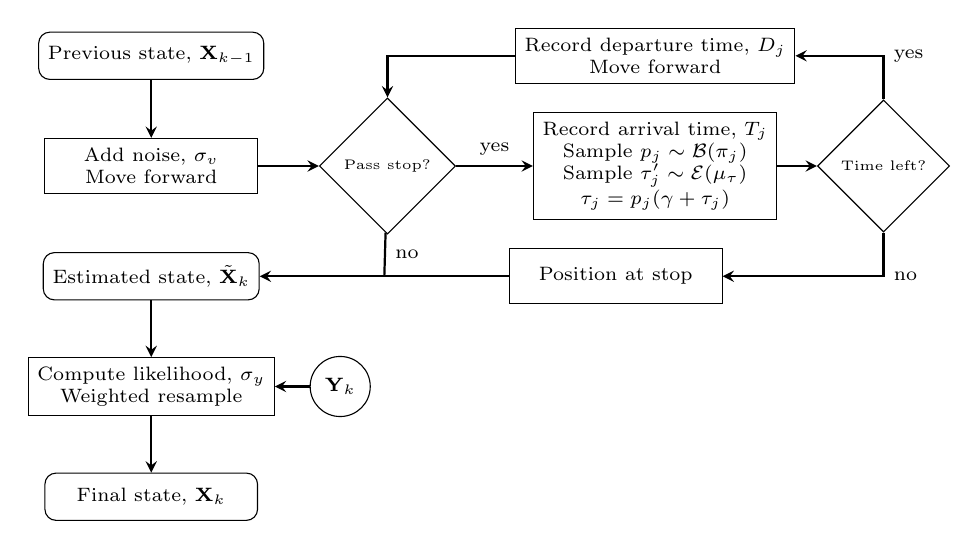
\begin{tikzpicture}[node distance=1.4cm]
    \node (start) [startstop] {Previous state, $\bX_{k-1}$};
    \node (move) [compute, below of=start,align=center] {Add noise, $\sigma_v$\\ Move forward};
    \node (stateEst) [startstop, below of=move] {Estimated state, $\tilde\bX_k$};
    \node (resample) [compute, below of=stateEst,align=center] %
    {Compute likelihood, $\sigma_y$\\Weighted resample};
    \node (end) [startstop, below of=resample] {Final state, $\bX_k$};

    \node (data) [data, right of=resample, xshift=1cm] {$\bY_k$};

    \node (passStop) [logic, right of=move, xshift=1.6cm] {\tiny Pass stop?};
    \node (arrival) [compute, right of=passStop, xshift=2cm, align=center]%
      {Record arrival time, $T_j$\\ Sample $p_j \sim \mathcal{B}(\pi_j)$\\%
      Sample $\tau_j' \sim \mathcal{E}(\mu_\tau)$\\$\tau_j = p_j(\gamma + \tau_j)$};
    \node (remaining) [logic, right of=arrival, xshift=1.5cm] {\tiny Time left?};
    \node (moveForward) [compute, above of=arrival, align=center]%
      {Record departure time, $D_j$\\Move forward};
    \node (stopped) [compute, below of=arrival, xshift=-0.5cm] {Position at stop};
    
    \draw [arrow] (start) -- (move);
    \draw [arrow] (stateEst) -- (resample);
    \draw [arrow] (data) -- (resample);
    \draw [arrow] (resample) -- (end);
    %\draw [arrow] (move) -- (stateEst);
    \draw [arrow] (move) -- (passStop);

    \draw [arrow] (passStop) -- node[anchor=south] {yes} (arrival);
    \draw [arrow] (arrival) -- (remaining);
    \draw [arrow] (remaining) |- node[anchor=west] {yes} (moveForward);
    \draw [arrow] (moveForward) -| (passStop);
    \draw [arrow] (remaining) |- node[anchor=west] {no} (stopped);
    \draw [arrow] (stopped) -- coordinate[midway] (toEst) (stateEst);
    \draw [line] (passStop) -- node[anchor=west] {no} (toEst);
  \end{tikzpicture}
  \caption{Diagram showing the logic included in the transition function (\vref{eq:particle_transition}) 
    for the proposed particle filter model, 
    using dwell time parameters defined in \cref{sec:bus-behaviour}.
    Actual dwell time is computed as the difference between departure and arrival times.
    $\mathcal{B}$ and $\mathcal{E}$ are the Bernoulli and Exponential distributions respectively.}
  \label{fig:pf_logic}
\end{figure}

In the particle filter model,
each particle is treated as an independent object with its own state.
Along with distance into trip and velocity (speed),
the state includes arrival times and dwell times at stops along the route,
yielding distributions at each stop which can then be used
as prior distributions for subsequent trips.
Over the course of a week, 
we can build up approximate distributions of dwell times for bus stops,
which we can then model based on time of day, day of the week,
and any other patterns we can detect.


It is hoped that the use of a \pf{} will overcome some of the issues
evident in the current system---including behaviour at loops---%
without too much additional effort.
On the downside, the \pf{} is significantly more demanding with respect to processing, 
so any models we do create will need to be computationally efficient
so they can process the real-time data from up to 1000~buses simultaneously.



\subsubsection*{Real-time Traffic State and Prediction}

Much of the research points out that knowledge of the current state of traffic
is fundamental to making accurate predictions \citep{yu-etal:2010,yu-etal:2011}.
We aim to develop a method of combining the real-time data from
all buses across Auckland
to produce a real-time ``map'' of the traffic conditions along bus routes.
Unlike previous examples,
we will not be restricting this to predefined routes that share common paths.


We will be using the state estimates from the \pf{} running on each active bus to infer
the general traffic conditions in the area.
This will be particularly useful during times of extreme or unusual congestion,
in which many road ways are likely to be affected,
even if routes do not overlap.
In turn, the information will also help to refine the estimates of speed in the \pf{}s,
further improving their accuracy.


Additionally, we intend to develop dwell time models for subsequent stops along a route
to further refine predictions.
This will range from the simpler models that use historical averages,
to more complex ones that can include interactions between routes.
For example, in some areas of Auckland,
there are several routes traveling down main roads heading into the city.
If the headway between two buses is small,
then we expect dwell times to be small too, since there has been less time for
new passengers to arrive at the stop.
\cite{hans-etal:2015} give several examples of models which use passenger
arrival rates to model dwell times.




\subsubsection*{Prediction Intervals and Journey Planning}

Communicating the results of our prediction models is important if they are to be of any use to anyone.
To makes things more interesting, the target audience is the general public,
who we do not assume to have any understanding of the technical terms we may be familiar with.
We intent to provide passengers with prediction intervals instead of point estimates,
which will allow us to convey uncertainty and 
solve the problem of ``increasing'' countdowns.


Since we will be using the particle filter to generate a prediction distribution,
obtaining intervals is as straightforward as in any other \gls{mcmc} application.
Therefore, we only need to focus on the quantiles used to obtain a prediction interval.
The intervals need to be small, 
but biased since, for a passenger, 
arriving early to a bus stop is favourable to arriving late and missing the bus altogether.
These predictions could then be made available through a simple web app,
displaying the \glspl{eta} of scheduled buses at a chosen stop.


A journey planning application will also be explored,
in which all of the information we have is compiled to assist passengers
in deciding on which bus to catch.
The three main categories for decisions are
(i) arrive before a given time, (ii) leave after a certain time,
and (iii) the fastest trip.
In all of these, the considerations are to reduce waiting time at the bus stop,
and in (i) to reduce the time between actual arrival and desired arrival;
of course, we need to account for uncertainty and minimise the probability of missing a bus
or being late in (i).
Since Auckland Transport will be simplifying fare structures so that they are not dependent 
on the route taken to get to your destination,
a ``lowest cost'' option that is available in some journey applications is redundant.


Over the coming years, Auckland Transport will be rolling out their new route structure,
which involve high-frequency local routes, 
with lower-frequency routes to connect the local ones.
As this happens, the journey planning application of our models will become more important,
since it will be of interest to passengers to minimise time waiting between transfers as well.



% ====================================================================================================== % INFO

% List \textit{specific} and \textit{new} results that your thesis
% plans to obtain, especially with regard to new statistical theory
% and methodology.
% It is essential that you have provided comprehensive background
% (in Section~\ref{sec:background})
% so that it is clear what new contributions will be made (here),
% and how they will extend what is currently known.
% Tie these with Appendix~A(i), and a list such as below is a
% good idea.


% For example, all of the points below are new (to my knowledge)
% and have not been done yet.
% \begin{enumerate}

% \item
% Develop a new method for quantile regression based on the
% asymmetric Laplace distribution and the concept of link functions
% and parallelism assumptions (via constraint matrices).


% \item
% Derive the asymptotic properties of the above method,
% both as $n \rightarrow \infty$ and as $p \rightarrow \infty$.




% \item
% Conduct a small simulation to check the mean squared error and
% other properties. To be done in R with some sections written in~C
% calling LINPACK \citep{dong:bunc:mole:stew:1979} for additional speed.



% \item
% Compare my results to those of~\cite{wei:carr:2009}, especially
% relating to boundary effects and small-sample properties.



% \item
% Tackle an important dataset or problem that no one has
% satisfactorily resolved before. It is essential that new
% methodologies are investigated and that novel insights are
% obtained. Note that a conventional analysis, even of a very large
% dataset, is \textit{not} PhD-level research.


% \end{enumerate}


% ----------------------------------------------------------------------
\section{Data and Special Needs}
\label{sec:data}

We will be working with the \gls{gtfs} real-time data provided through Auckland Transport's
\gls{api}, available from \url{https://dev-portal.at.govt.nz}.
\gls{gtfs} is a specification developed by Google,
and provided as a way for transit organisations to provide transit data to developers
\citep{gtfs}.
It consists of the static component, which contains schedule information and route shapes,
and the real-time component, which provides,
along with other information,
the real-time \gls{gps} locations of vehicles.


The \gls{gtfs} static feed is a set of files, available as a single ZIP archive,
that contains the latest schedule information, including trips, routes, shapes, stop times,
and calendar timetables.
A ``trip'' is a single journey at a specific time of day,
with a set of stops and the associated arrival and departure times at them.
A ``route'' is a specified sequence of stops,
and can have multiple trips per day.
Each route has a ``shape'', which is a sequence of latitude and longitude coordinates
describing the path of the vehicle.
Other information, such as calendars, allow us to know ahead of time which trips
are (and are not) scheduled on a particular day,
such as public holidays.


The \gls{gtfs} real-time feed consists of \gls{gps} locations,
which are updated usually every 30~seconds.
Therefore, we need to re-run all of our computations and update predictions approximately
every 30~seconds, which means we will require the computational power to do so.
We will need a dedicated machine capable of
retrieving the data, analysing it, and making predictions,
as well as a web server to make these predictions available to passengers.
The exact requirements will depended on the demands of the state and prediction models,
although we intend for the requirements to be as low as possible
to allow our model to be deployed to other \gls{gtfs} systems easily.


% ====================================================================================================== % INFO

% Almost all Statistics PhD theses should analyse at least one
% data set, even if it is a toy data set.


% State their source fully.
% If new data is important to the thesis describe what's new.
% Why is this data set important?
% What is novel about it?
% Specify any ethics or confidentiality issues.


% A plot of some of the data may be useful;
% see Figure~\ref{fig:myfig}.


% Do you have any special needs such as IT needs?
% These include hardware (supercomputing facilities),
% and expertise/technical knowledge.
% Often extra large data sets have special needs associated
% with its processing.
% How do you invisage those needs to be met?



% Funding: anything to report here?
% If your thesis work involves experiments, travel or special
% resources in order to collect data, or essential collaboration with
% experts in your field, then you should describe these requirements
% here along with how you, or your supervisor, will fund these
% requirements. Departments work on tightly planned budgets and
% generally do not have the facilities to pay for unplanned PhD
% related expenses.



% If ethics approval(s)/permissions is needed then put
% any details here.





% \begin{figure}[tt]
% \begin{center}
% %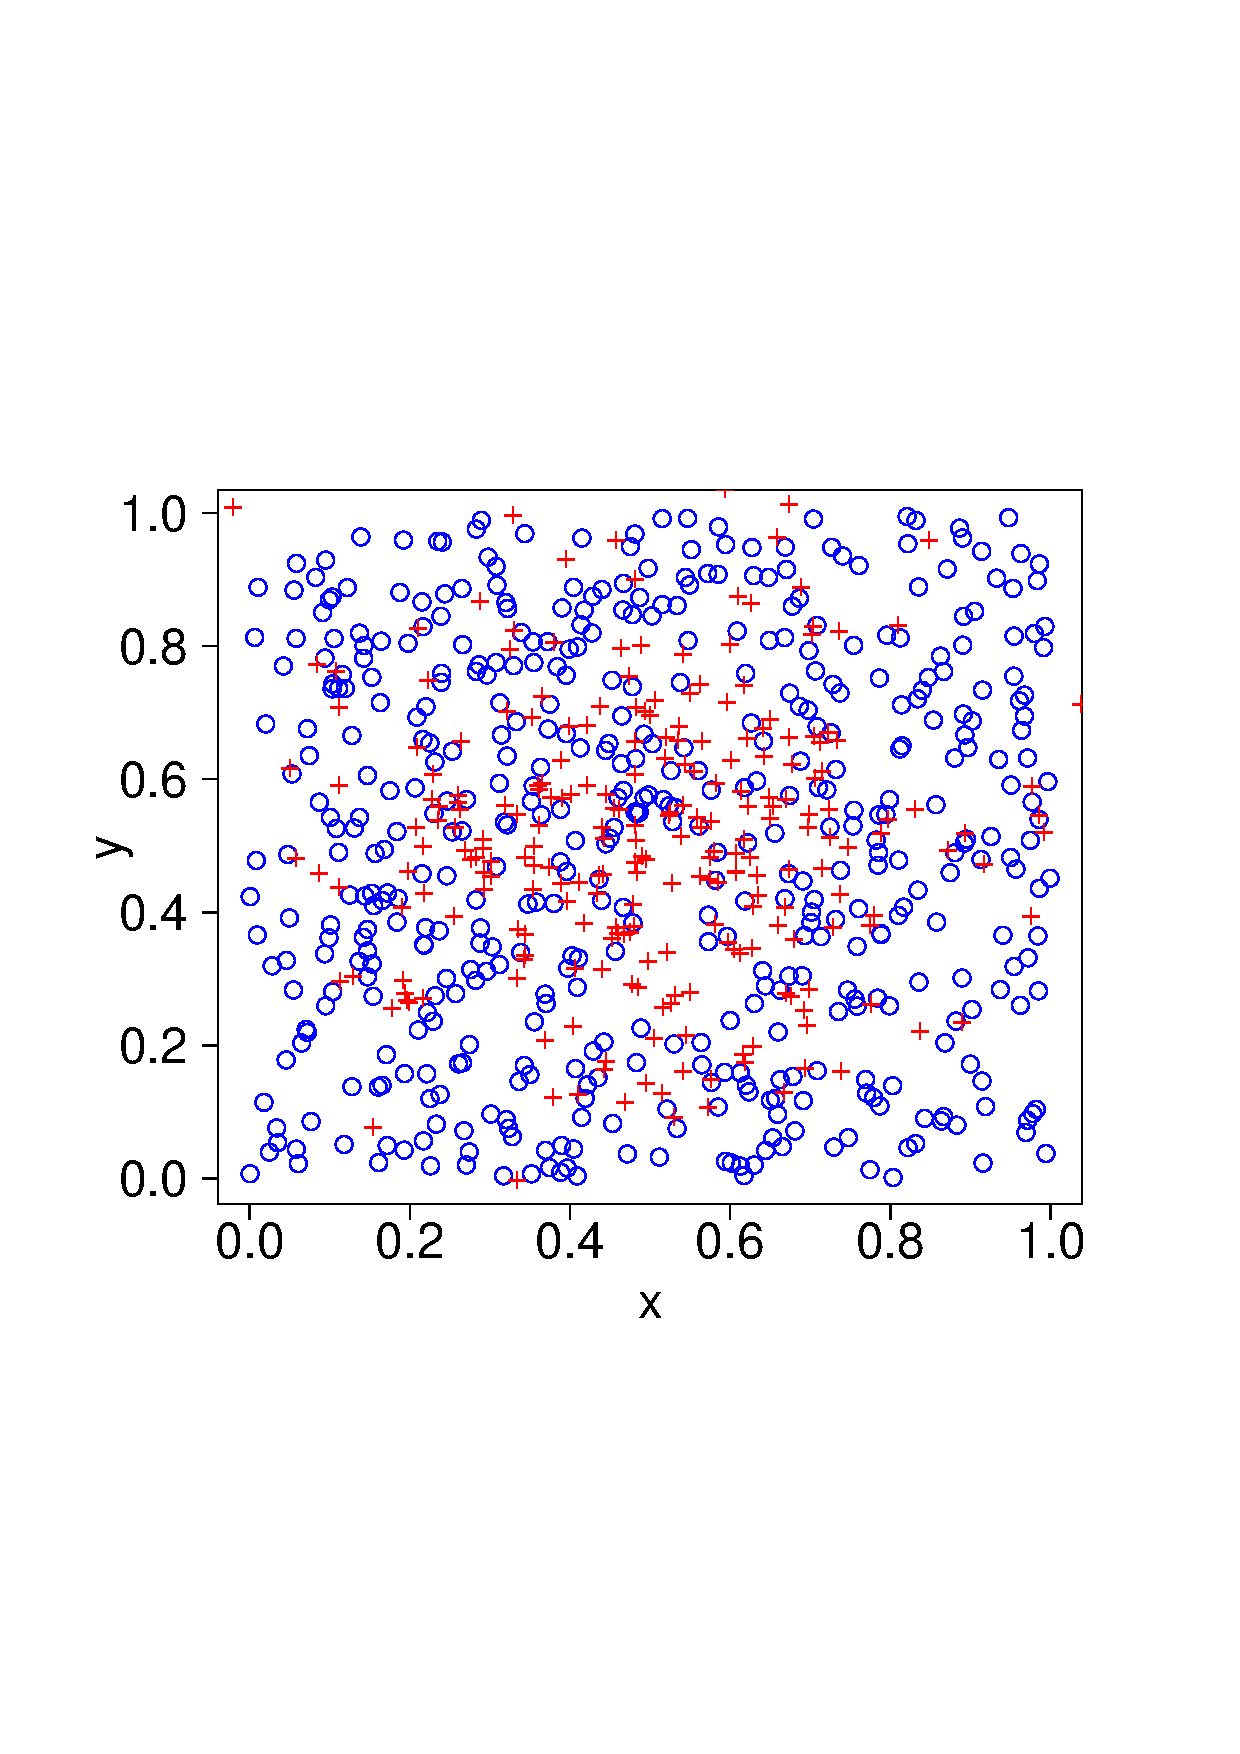
\includegraphics[height=70mm]{./myfig.pdf}
% \caption{
% Data for a two-class classification problem.
% The red ``+'' is for class~1, and $n = 250$.
% The blue ``o'' is for class~2, and $n = 500$.
% }
% \label{fig:myfig}
% \end{center}
% \end{figure}



% ----------------------------------------------------------------------
\section{Goals}

% ====================================================================================================== % INFO

% List \textit{specific} goals you wish to achieve in your PhD.


% \begin{enumerate}

% \item
% I wish to derive the first three moments of the Slash distribution.
% This will involve working out the characteristic function first.


% \begin{itemize}

% \item[a.]
% Then work out the observed information matrix
% based on~\cite{bick:etal:2009}.

% \item[b.]
% Then work out the expected information matrix
% \citep{scot:lee:wild:2007}.

% \item[c.]
% Apply the EM algorithm \citep{demp:lair:rubi:1977} to estimate~$\lambda$.

% \item[d.]
% Write a R package to implement my method.
% It will be written in S4 and use object oriented methods
% \citep{cham:1998}.

% \item[e.]
% Apply the method to the radiation data set
% \citep{MR2526777}.

% \item[f.]
% Extend biplots \citep{gowe:1966} for my data.

% \item[g.]
% Release the package on CRAN
% (cf.~\cite{murr:ihak:2000}).

% \item[h.]
% Publish my results in at least two papers,
% earmarked for JASA and JRSS-B.
% Also an applications paper in Biometrics.
% See Section~\ref{sec:timeline}.

% \end{itemize}



% \item
% Solve the Fisher-Behrens problem
% \citep{efro:2009,MR2415600,MR2508377}.


% \end{enumerate}

% ====================================================================================================== %

\begin{enumerate}
\item
  Implement a \pf{} on a small collection of routes in Auckland and explore prediction methods.

\item
  Use travel times of recent trips to predict arrival times,
  and compare this to using solely historical data, as well as a combination of both.

\item 
  Find a collection of routes using the same paths and explore methods of using the speed information,
  without requiring manual specification.

\item
  Compare different summary statistics and prediction intervals;
  use ``simulations'' to determine actual versus predicted wait times.

\item
  Use a large collection of routes to implement the model, and assess the performance of the model. 
  If necessary, explore methods of optimisation.

\item
  Make a simple web application that allows users to easily get arrival time predictions for their bus.
  
\item
  Package the system so that it is distributable to other \gls{gtfs} feeds,
  and so that it is not dependent on us.

\end{enumerate}






% ----------------------------------------------------------------------
\section{Timeline and Activities}
\label{sec:timeline}

% ====================================================================================================== % INFO

% \begin{table}[hh]
% \caption{
% Timeline of my privisional year.
% }
% \centering
% \ ~~~~ \\
% \label{tab:timeline}
% \begin{tabular}{cl}
% \toprule
% Date & Activity \\
% \midrule
% 2010-04-01 & Provisional PhD registration (PhD in Statistics). \\
% 2010-05-01 & Updated my personal webpage at
%              \textsf{www.stat.auckland.ac.nz/$\sim$tell029}. \\
% 2010-05-20 & Attended one of the
%              Doctoral Skills Programme's Induction Days. \\
% 2010-09-01 & Gave my first talk at NZSA conference. Won first prize. \\
% 2010-11-01 & Gave a talk to PhD Talks Day. \\
% 2011-01-15 & Submit my first paper to \textit{Annals of Statistics}
%              (co-authored with supervisor). \\
% 2011-05-01 & Presented my research progress to a departmental seminar. \\
% 2012-01-20 & Achieve Goal~1. \\
% 2012-08-20 & Achieve Goal~2. \\
% 2012-10-23 & Submit my second paper to \textit{Annals of Applied Statistics}
%              (co-authored with supervisor). \\
% 2013-01-15 & Submit my third paper to \textit{Biometrics}
%              (sole authorship). \\
% 2013-02-01 & Submit my PhD thesis. \\
% \bottomrule
% \end{tabular}
% \end{table}

% ====================================================================================================== %

I have fulfulled almost all of my first year requirements.
These are:
\begin{enumerate}

\item
All EoI provisional goals:
\begin{enumerate}

\item
\textit{Approval of the full thesis proposal by the appropriate departmental/faculty postgraduate
committee}:
In progress

\item
\textit{A substantial piece of written work, such as a literature review, completed to the
satisfaction of the main supervisor}: Section~2


\item
\textit{Presentation of the proposal and/or work in progress to an appropriate forum e.g.\ seminar,
research group, conference, to the satisfaction of the supervisors}:
2016-08-17

\item
\textit{Attendance at one of the Doctoral Skills Programme
Induction Days}:
2015-11-04

\item
\textit{Successful completion of the Academic Integrity Module}:
completed with MSc, 2014

\item
\textit{Undertake Diagnostic English Language Needs Assessment (DELNA) online screening}:
25/02/2010

\item
\textit{Complete STATS 710 and STATS 769 at B+ or higher grade within the first
12~months of registration}\\
B in STATS~710; STATS~769 will be completed at the end of semester 2, 2016.

\item
\textit{Attendance of at least 10~Statistics departmental research seminars per annum,
with forms fully filled in and handed in}:
see Table~\ref{tab:seminars}

\item
\textit{Maintenance of a personal departmental webpage providing information on scholarly
activities and objectives to the satisfication of the supervisor and Department of Statistics
PhD Officer}:
\url{https://www.stat.auckland.ac.nz/people/tell029}

\item
\textit{Satisfactory participation in the Department of Statistics PhD Talks Day and/or give
a departmental seminar within the first 12~months of registration}:
presenting on 17-08-2016


\end{enumerate}





% \item
% I have updated my webpage
% (\textsf{www.stat.auckland.ac.nz/$\sim$myStudentName})
% giving details of my thesis, links to other research resources
% in my topic, and some personal stuff to make it interesting.


% \item
% I have diligently attend as many Statistics Department seminars
% as I could. They are given in Table~\ref{tab:seminars}.
% This is much more than the minimum quota set by the department.
% Consequently there should be no problem due to this when getting
% my annual report signed off\footnote{If insufficient seminars have
% been attended then sign off will occur \textit{after} the minimum number
% is reached.}.
% The 2010-04-08 seminar was particularly useful because it gave
% me an idea on how to solve one of my problems.


% \item
% I did STATS~730 in Semester~1 of 2010 and obtained an A+.


% \item
% I did STATS~782 in Semester~2 of 2010 and obtained an A.



\end{enumerate}



\begin{table}[hh]
\caption{
Departmental seminars I have attended.% (top part of the table).
%Talks from another UoA departments are in the middle tier.
%Conferences and workshops are in the bottom tier.
}
\centering
\ ~~~~ \\
\label{tab:seminars}
\begin{tabular}{cll}
\toprule
Date & Speaker & Title \\
\midrule
2015-09-02 & Moshe Haviv &
Queues \& cooperative games \\
%
2015-11-18 & Hadley Wickham &
Pure, predictable, pipeable: creating fluid interfaces with R \\
%
2016-01-16 & Xudong Huang &
Composite likelihood estimators, mixed models \& complex \\
&&sampling \\
%
2016-01-27 & Kevin Knuth &
Modern probability theory \\
%
2016-01-28 & Maartje an de Vrugt &
Online appointment scheduling: a taxonomy and review \\
%
2016-02-24 & Arndl von Haeseler &
Terraces, partial terraces, and phylogenetic inference \\
%
2016-03-31 & Shengwei Hu &
Classification on high-dimensional data using\\&&nonparametric mixtures \\
%
2016-04-14 & June Lau &
Optimizing the cardiac patient's journey: using mathematical \\
&&modelling to guide patient flow, staffing, scheduling and \\
&&resource allocation through the cardiac unit \\
%
2016-06-01 & Arman Bilge &
Hamiltonian Monte Carlo on the space of phylogenies \\
%
2016-07-13 & Nikki Sonenberg &
Matrix analytic methods for analysing stochastic fluid models \\
%
% \midrule
% 2010-06-16 & James B.~Conant &
% ``Geography is not a university subject'' (geo Department) \\
% %
% yyyy-mm-dd & Speaker Name &
% Title of Talk \\
% \midrule
% 2010-05-29 & David Siegmund &
% Workshop on `Genetic Mapping' at UoA. \\
%
\bottomrule
\end{tabular}
\end{table}




% ----------------------------------------------------------------------
\section{Summary}



% Give a few sentence summary of your thesis, especially
% what's new.

The estimation of future arrival times is a difficult task,
especially when we are unable to directly measure many of the 
variables that contribute to delays in the system.
We anticipate that the use of a \pf{} as a real-time model will
help us to overcome many of the major sources of error in the system,
as well as handle situations that may confuse current models.
Further, by combining the estimated states of all buses,
we hope to get a real-time picture of the state of traffic along bus routes throughout Auckland,
allowing us the make more accurate---and precise---predictions,
which can then be made available to passengers.




% ----------------------------------------------------------------------
% \section*{Appendix~A}

% Delete or replace the contents of this section with any
% appendices you may have.

% \bigskip

% \bigskip

% The \textit{University of Auckland Statute and Guidelines for the
% Degree of Doctor of Philosophy (PhD)} (2008)
% reads\footnote{Clause~1, Preamble, item~(d).}:

% \bigskip


% \noindent
% ``The PhD degree is awarded for a formal and systematic
% exposition of a coherent programme of advanced research
% work carried out over the period of registration for the
% degree which in the opinion of the examiners and the Board
% of Graduate Studies satisfies all of the following criteria:

% \begin{itemize}

% \item[(i)] to be an original contribution to knowledge or
% understanding in its field, and

% \item[(ii)] to meet internationally recognised standards
% for such work, and

% \item[(iii)] to demonstrate a knowledge of the literature
% relevant to the subject and the field or fields to which
% the subject belongs, and the ability to exercise critical
% and analytical judgement of it, and

% \item[(iv)] to be satisfactory in its methodology, in the
% quality and coherence of its written expression, and in
% its scholarly presentation and format.''

% \end{itemize}




\vfill\pagebreak
\addcontentsline{toc}{section}{References}
\bibliographystyle{./elsart-harv} % elsart-harv,plain,unsrt,alpha
\bibliography{./myrefs}


\end{document}
